%*******************************************************
% Capitulo cinco
%*******************************************************
\chapter{Capa motivacional y de despliegue}

\section{Stakeholders}

\marginpar{\begin{figure}[H]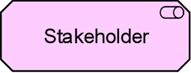
\includegraphics[scale=0.8]{istakeholder}\end{figure} \footnotesize \textbf{Stakeholder}. El rol de un individuo, equipo, o organización (o alguna clase de ellas) que representa sus intereses en, o su relación con, el resultado de la arquitectura.\\}

\marginpar{\begin{figure}[H]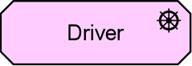
\includegraphics[scale=0.8]{idriver}\end{figure} \footnotesize \textbf{Manejador}. Algo que crea, motiva y alimenta el cambio en la organización.\\}

El punto de vista de los Stakeholders permite modelar las partes interesadas, los manejadores internos y externos, y las evaluaciones (en términos de fortalezas, debilidades, oportunidades y amenazas) de estos manejadores. Además, también modela los vínculos con los objetivos iniciales (de alto nivel) y las valoraciones que puedan ser descritas. Estos objetivos constituyen la base para el proceso de ingeniería de requisitos, incluyendo el refinamiento de los objetivos, análisis de conflictos y contribuciones, y la derivación de los requisitos que realizan los objetivos.

\begin{figure}[H]
\centering
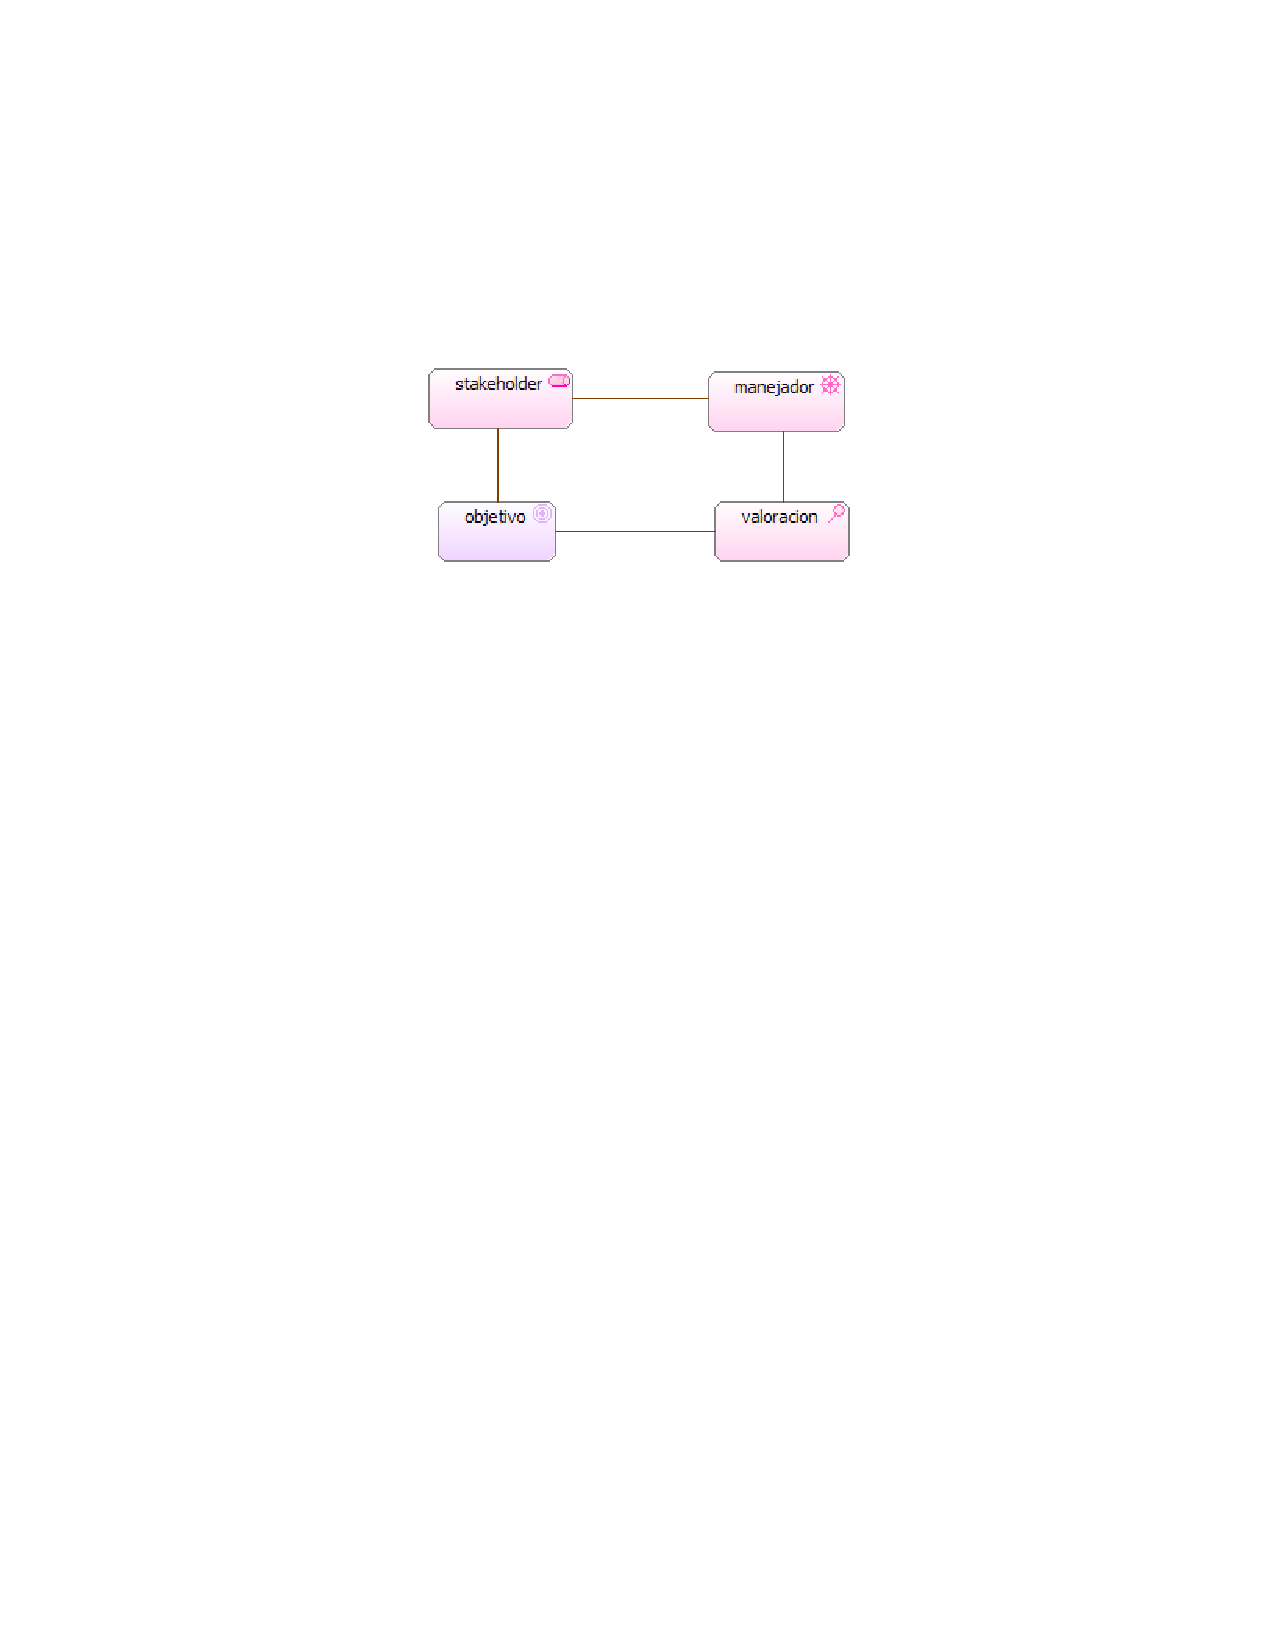
\includegraphics{stakeholder}
\caption{Metamodelo del punto de vista de stakeholder.}
\end{figure}

\marginpar{\begin{figure}[H]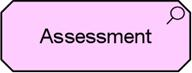
\includegraphics[scale=0.8]{iassessment}\end{figure} \footnotesize \textbf{Valoracion}. El resultado de un análisis de algún manejador.\\}

\marginpar{\begin{figure}[H]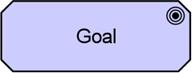
\includegraphics[scale=0.9]{igoal}\end{figure} \footnotesize \textbf{Objetivo}. Un estado final que un stakeholder pretende alcanzar.}

En esta propuesta los Stakeholders externos son los Clientes, Usuario final, Proveedores de servicios de TI, Proveedores de servicios de ads, Consultores y Socios de negocios. Los Stakeholders internos son Gestores de conocimiento, Directores de producto y Directores de cuenta. Algunos de ellos se relacionan con Manejadores (Drivers) los cuales impulsan los objetivos. Una vista de los Stakeholders principales de este negocio puede verse en la figura \ref{diagramastakeholders}, la cual refleja algunos de los cuadrantes del modelo canvas.

\begin{figure}[H]
\centering
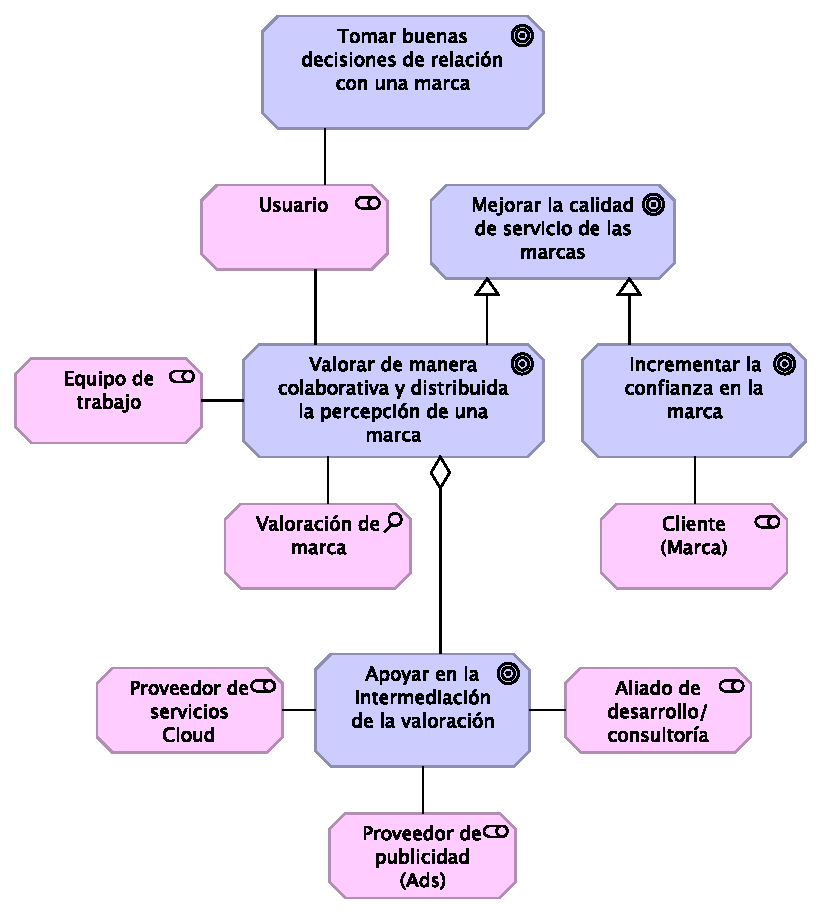
\includegraphics[scale=0.85]{Mstakeholders}
\caption{Punto de vista de stakeholder.}
\label{diagramastakeholders}
\end{figure}

El objetivo es la Mejora de la calidad en el servicio de las marcas. Que se especializa en dos objetivos importantes: Valorar de manera colaborativa y distribuida las marcas e Incrementar la confianza en la marca, este último ejecutado por el equipo de trabajo; y el objetivo de Incrementar la confianza en la marca, ejecutado por el cliente mismo. Otros stakeholders como los proveedores o alidados, descritos en el canvas, apoyan el objetivo de la intermediación en la valoración. 

\section{Realización de objetivos}

El punto de vista de realización de objetivos permite modelar el refinamiento de los objetivos (de alto nivel) en objetivos más concretos, y el refinamiento de objetivos concretos en requisitos o condiciones que describen las propiedades que son necesarias para alcanzar los objetivos. 

El refinamiento de objetivos en sub-objetivos se modela utilizando relaciones de agregación. El refinamiento de las metas en los requerimientos se modela utilizando la relación de realización. Además, los principios pueden ser modelos que guían el refinamiento de los objetivos soportándose con los requisitos.

\begin{figure}[H]
\centering
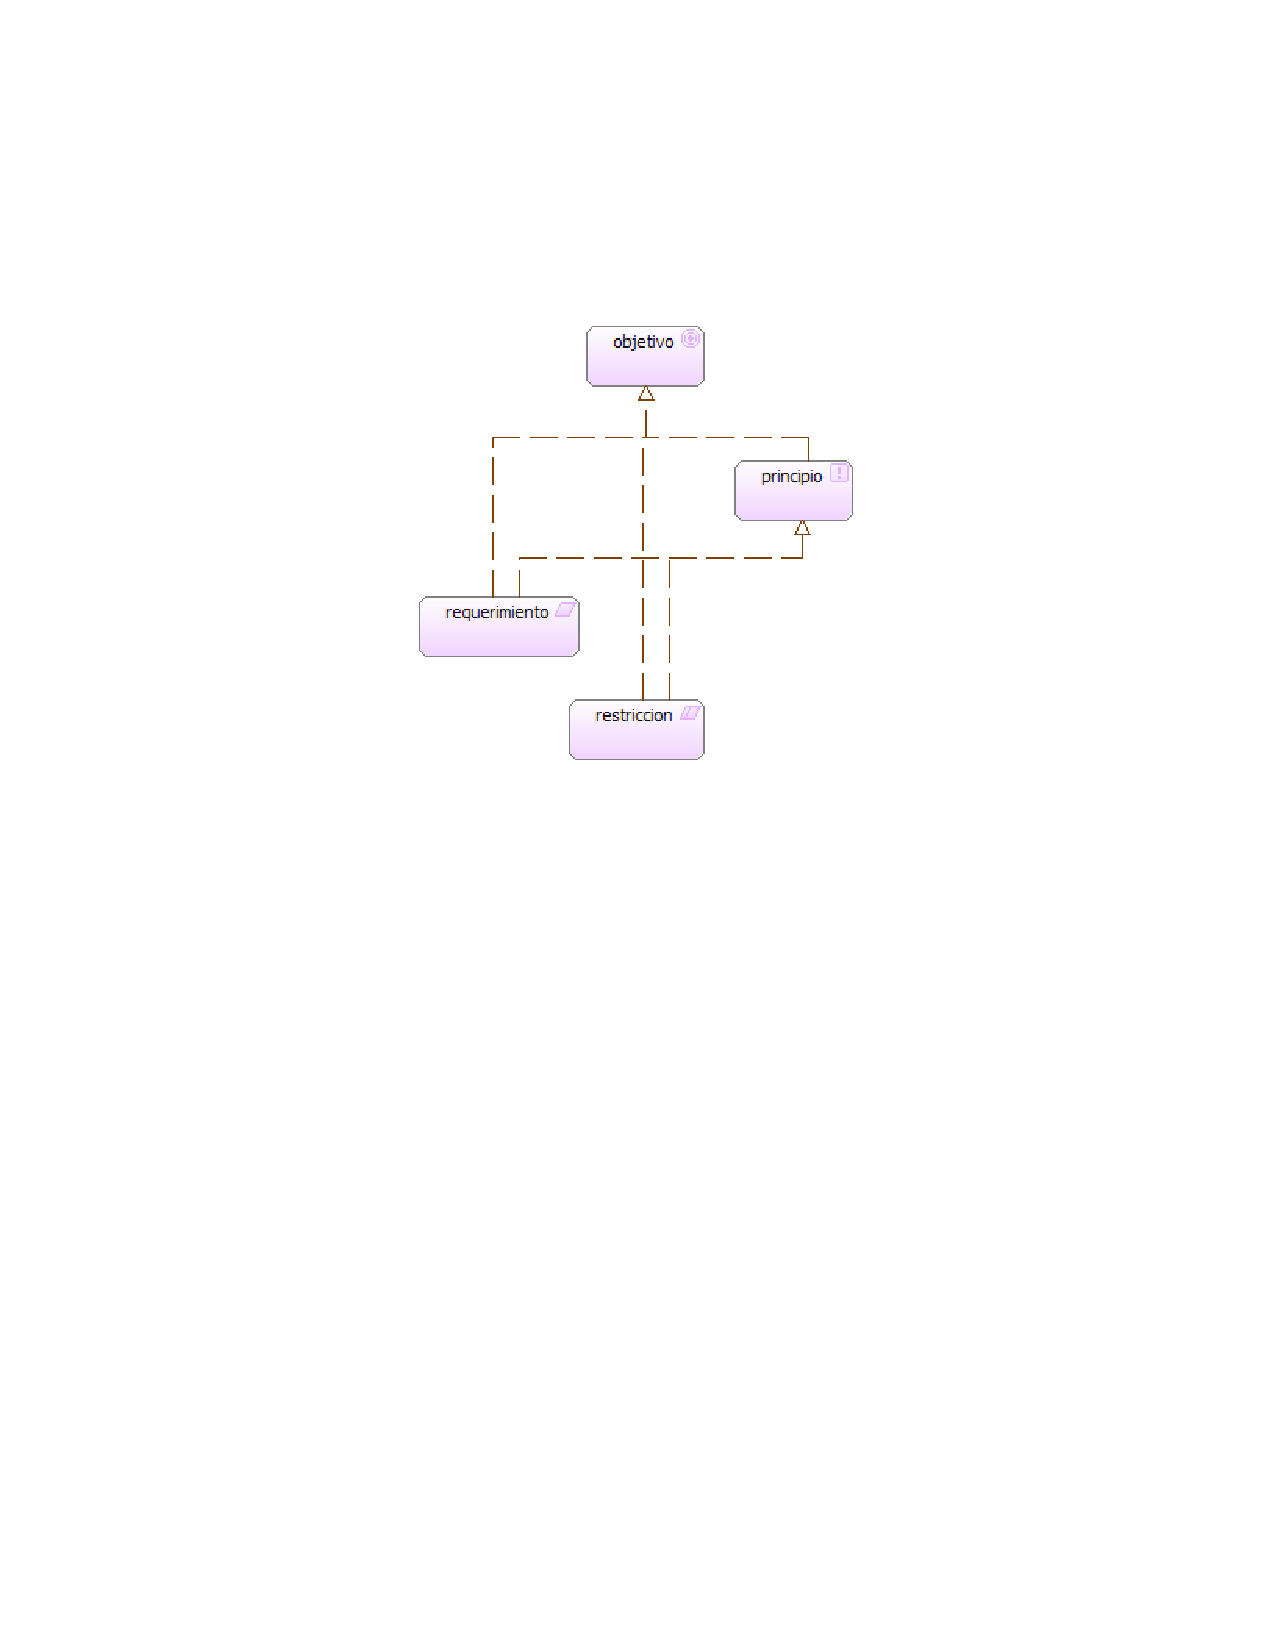
\includegraphics[scale=0.9]{realizacion_de_objetivos}
\caption{Metamodelo del punto de vista de realización de objetivos.}
\end{figure}

\marginpar{\begin{figure}[H]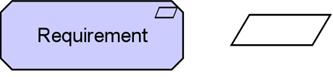
\includegraphics[scale=0.7]{irequeriment}\end{figure} \footnotesize \textbf{Requerimiento}. Una necesidad que debe ser realizada por un sistema.\\}

\marginpar{\begin{figure}[H]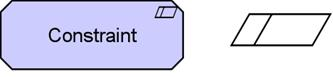
\includegraphics[scale=0.7]{iconstraint}\end{figure} \footnotesize \textbf{Restricción}. Restricción en la forma que un sistema debe ser realizado.}

La realización de objetivos nos muestra algunos de los requisitos más importantes que deben ser creados: la valoración de las marcas, la comparación y la gestión de información de la marca. Una restricción importante es lograr una valoración cuantitativa que permita hacer la comparación.

\begin{figure}[H]
\centering
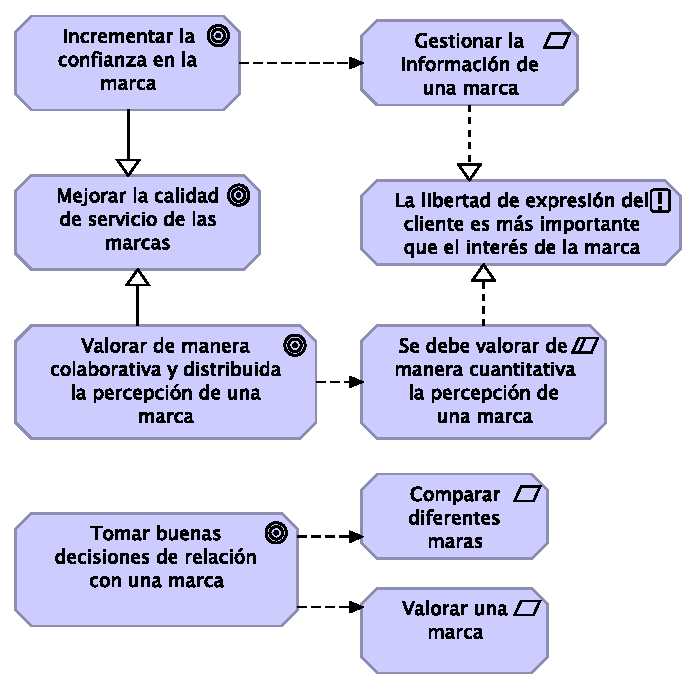
\includegraphics[scale=1]{MRealizaciondeobjetivos}
\caption{Punto de vista de realización de objetivos.}
\end{figure}

\section{Contribución de objetivos}
El punto de vista de contribución de objetivos permite a un diseñador o analista modelar las relaciones que influyen entre los objetivos y requisitos. El resultado de este punto de vista se puede utilizar para analizar el impacto que tienen sobre los objetivos entre sí o para detectar conflictos entre los objetivos de las partes interesadas. Por lo general, este punto de vista se puede utilizar después de  que los objetivos han, en cierta medida, sido refinados en sub-objetivos y, posiblemente, en requisitos. Por lo tanto, las relaciones de agregación y de realización también se puede mostrar en este punto de vista.

\begin{figure}[H]
\centering
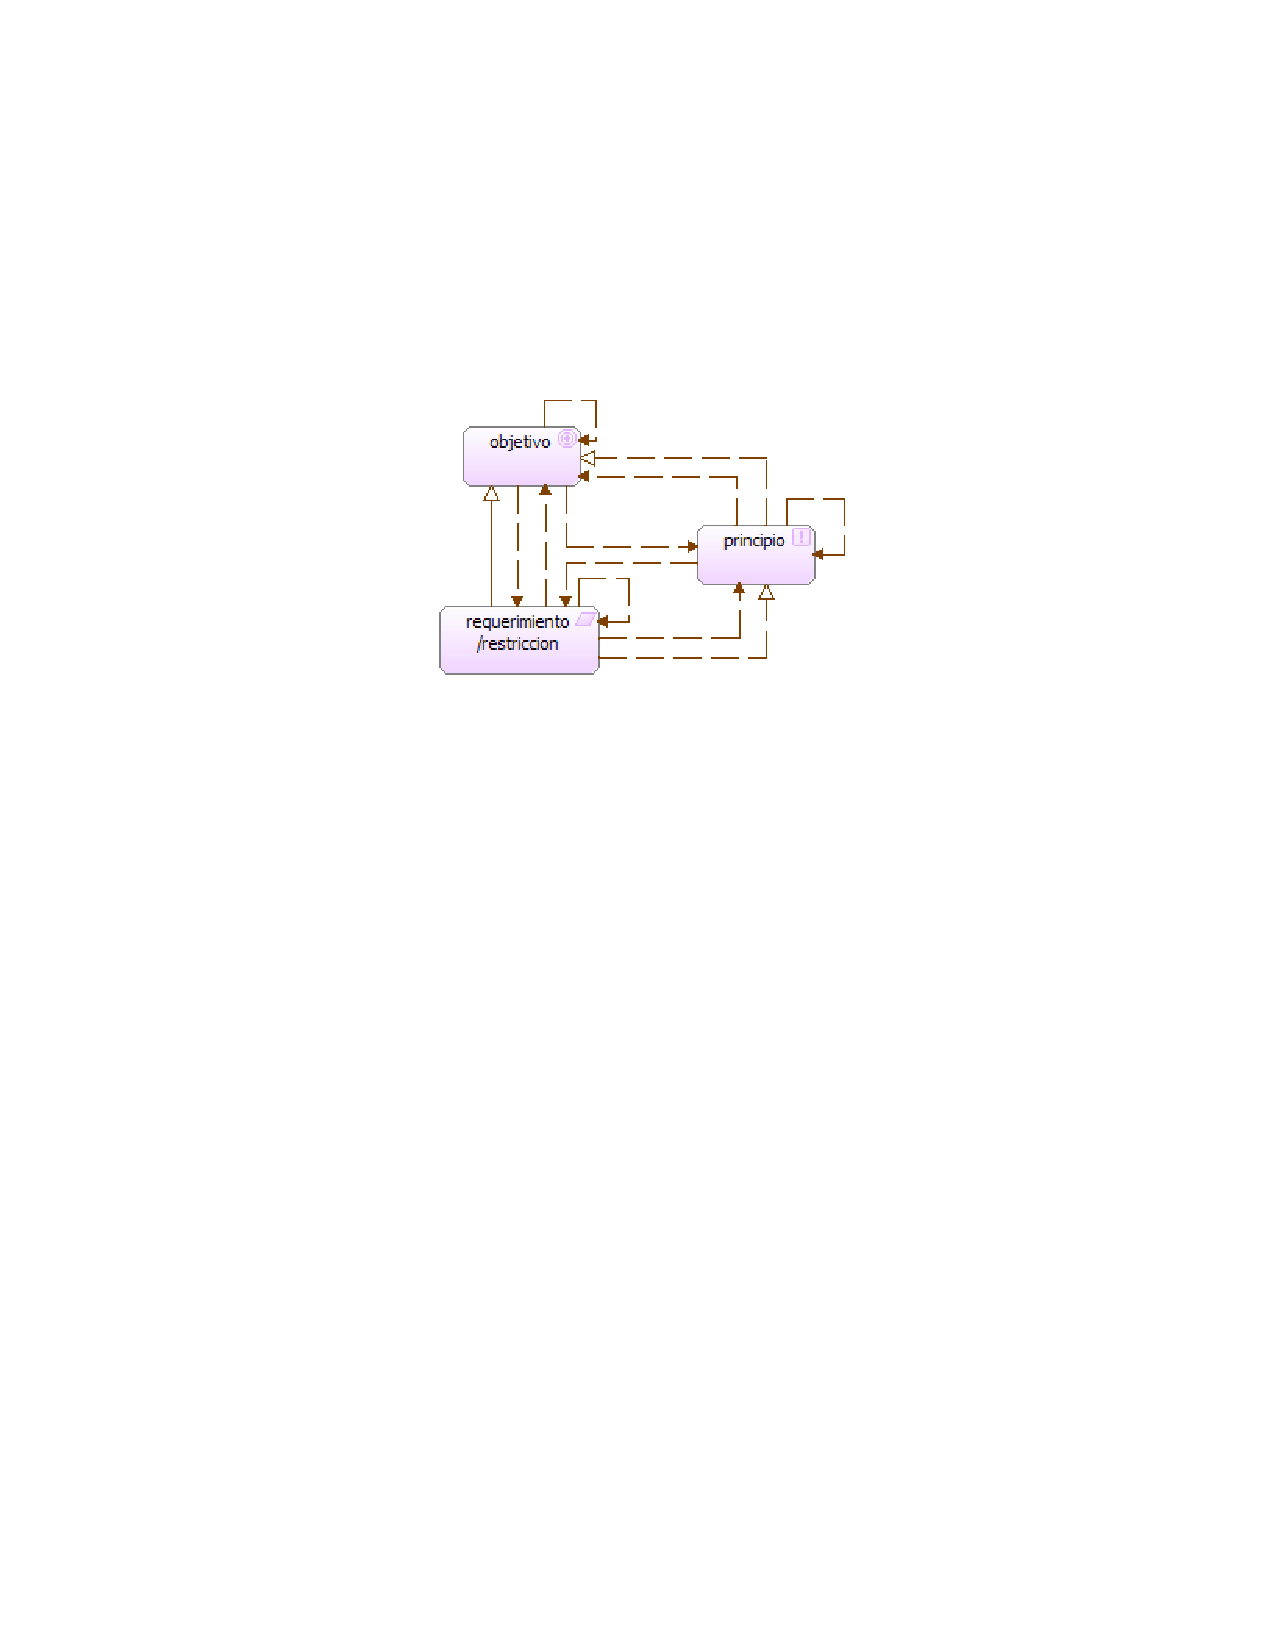
\includegraphics{contribucion}
\caption{Metamodelo del punto de vista de contribución de objetivos.}
\end{figure}

Es de destacar que en la presente propuesta el objetivo de mejorar la calidad de servicio de las marcas es afectado por el requerimiento de comparar diferentes marcas. Esta situación ocurre bajo la consideración que el usuario puede escoger de manera libre el mejor prestador del servicio al poder hacer la comparación. Una vez las marcas entienden que pueden ser escogidas de acuerdo a la percepción difundida y usada para la comparación mejorarían su servicio.

\begin{figure}[H]
\centering
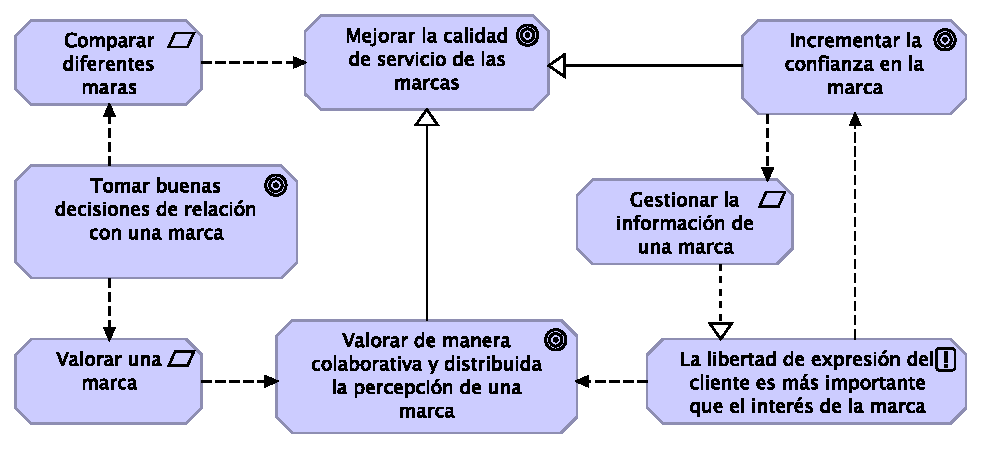
\includegraphics[scale=0.8]{MContribucion}
\caption{Punto de vista de contribución de objetivos.}
\end{figure}

\section{Principios}

\marginpar{
    \begin{figure}[H]
        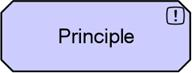
\includegraphics[scale=0.8]{iprinciple}
    \end{figure} 
    \footnotesize 
    \textbf{Principio}. Una propiedad normativa de todos los sistemas en un contexto dado, o la forma en que se realizan.
}

El punto de vista de los principios permite al analista o diseñador modelar los principios que son relevantes para diseñar el problema a mano, incluyendo los objetivos que motivan a estos principios. Además, las relaciones entre los principios y sus objetivos, pueden ser modelados. Por ejemplo, los principios pueden influir entre sí positiva o negativamente.

\begin{figure}[H]
\centering
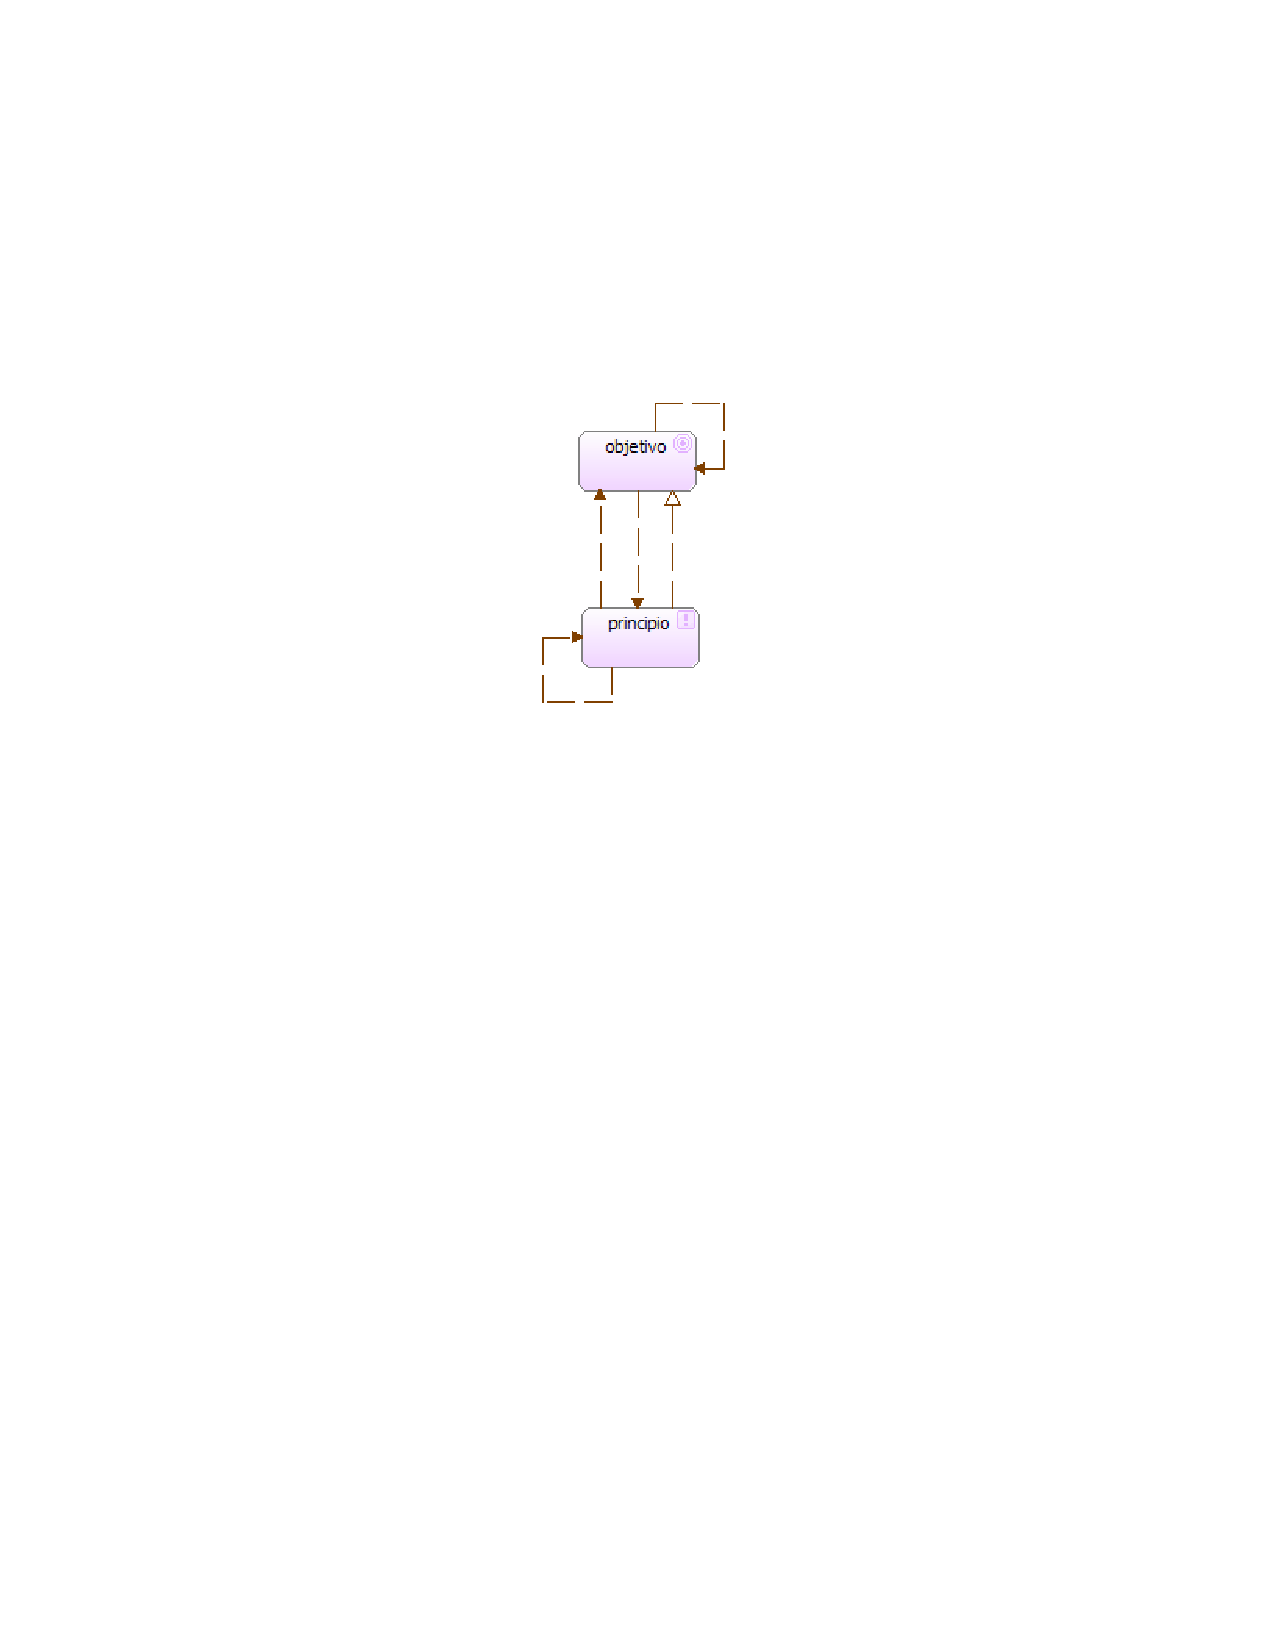
\includegraphics[scale=0.8]{principios}
\caption{Metamodelo del punto de vista de principios.}
\end{figure}

El principio principal es que \textit{La libertad de expresión del cliente es más importante que el interés de la marca}. Tiene un significado muy importante: el diseño de la aplicación es principalmente para beneficiar al usuario con información de calidad sin censura.

\begin{figure}[h]
\centering
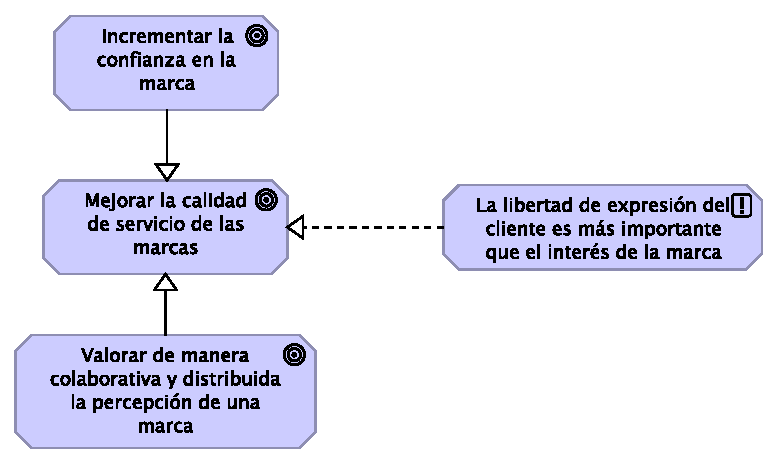
\includegraphics[scale=1]{MPrincipios}
\caption{Punto de vista de principios.}
\end{figure}


\section{Realización de requisitos}

El punto de vista de realización de requisitos permite al diseñador modelar la realización de los requisitos por parte de los elementos básicos, tales como agentes de negocios, servicios de oficina, los procesos de negocios, servicios de aplicaciones, componentes de la aplicación, etc. Por lo general, los requisitos resultan del punto de vista de refinamiento de los objetivos. Además, puede ser usado para refinar requisitos en requisitos más detallados. La relación de agregación se usa para este propósito.

\begin{figure}[h]
\centering
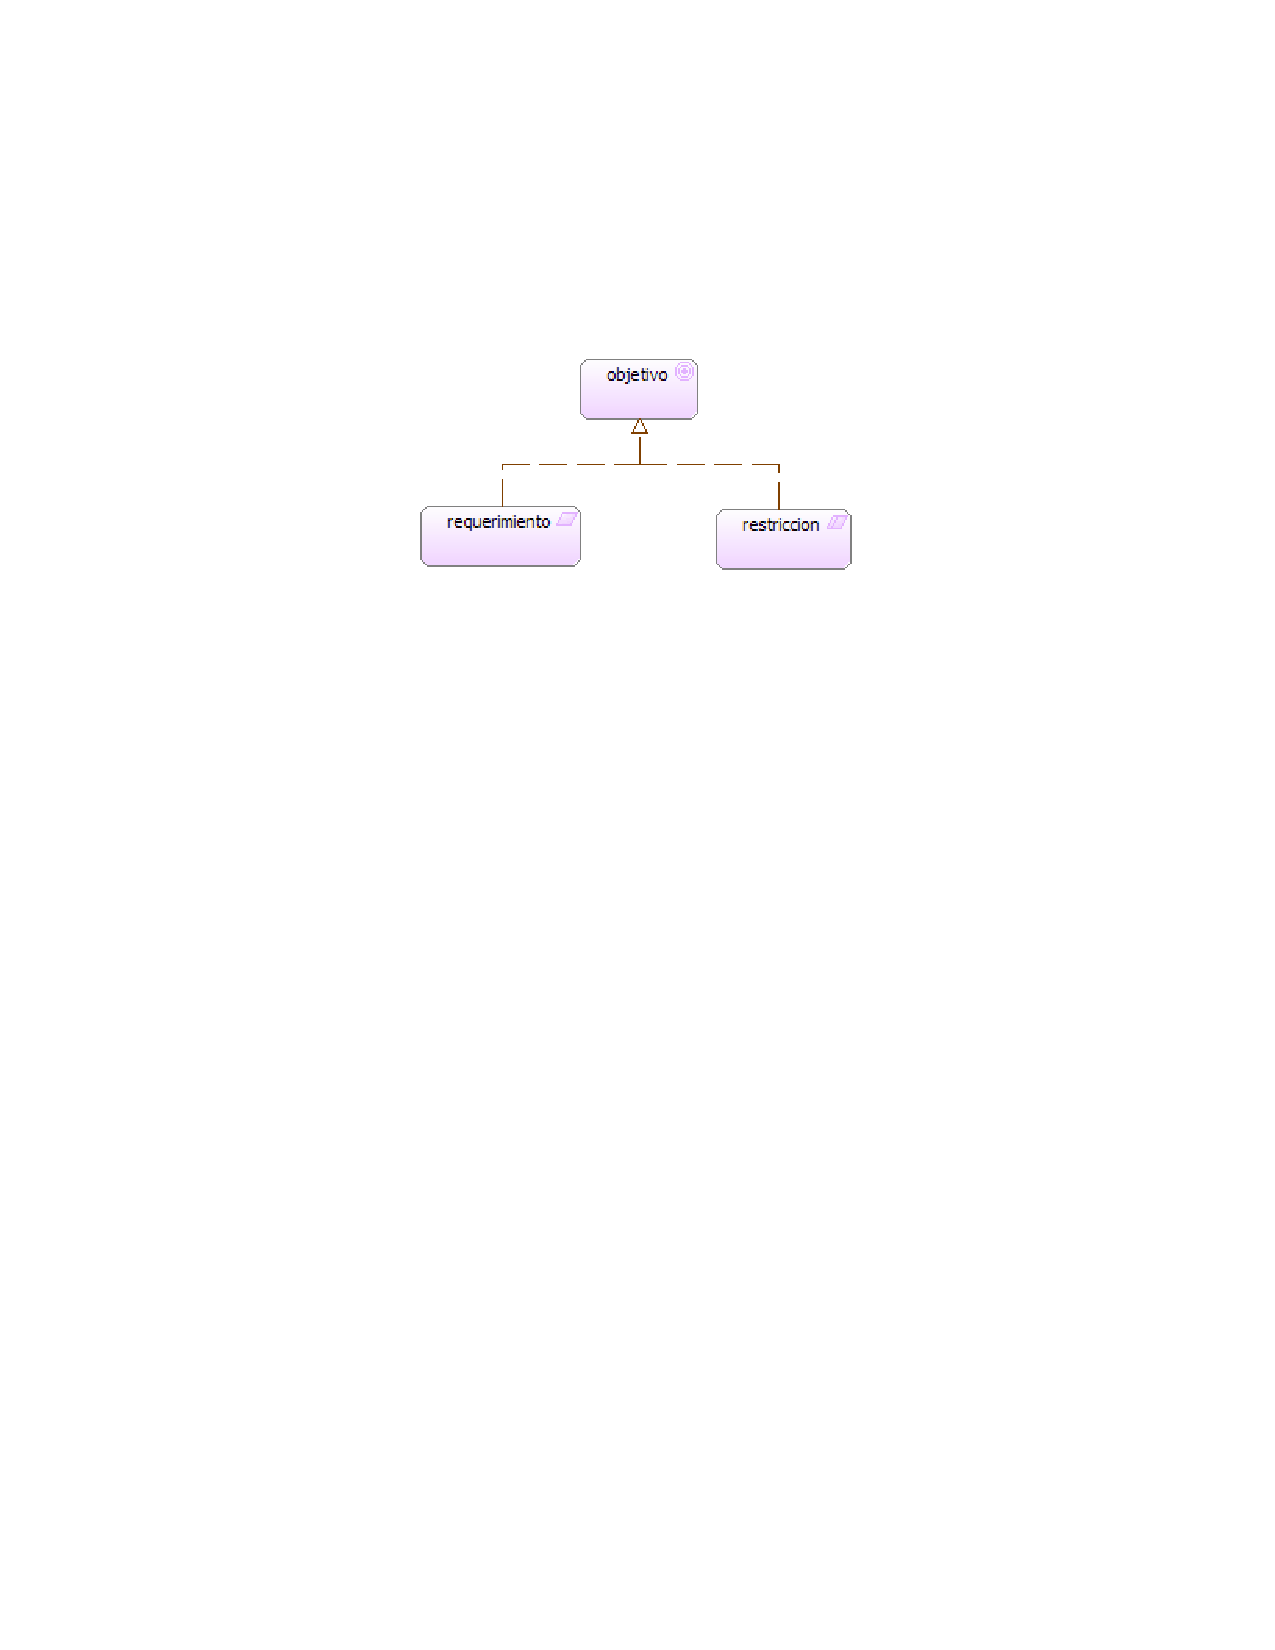
\includegraphics{realizacion_de_requerimientos}
\caption{Metamodelo del punto de vista de realización de requisitos.}
\end{figure}

Los requisitos que realizan a los objetivos más importantes se materializan en tres: Valorar una marca, comparar diferentes marcas y gestionar la información de una marca.

\begin{figure}[h]
\centering
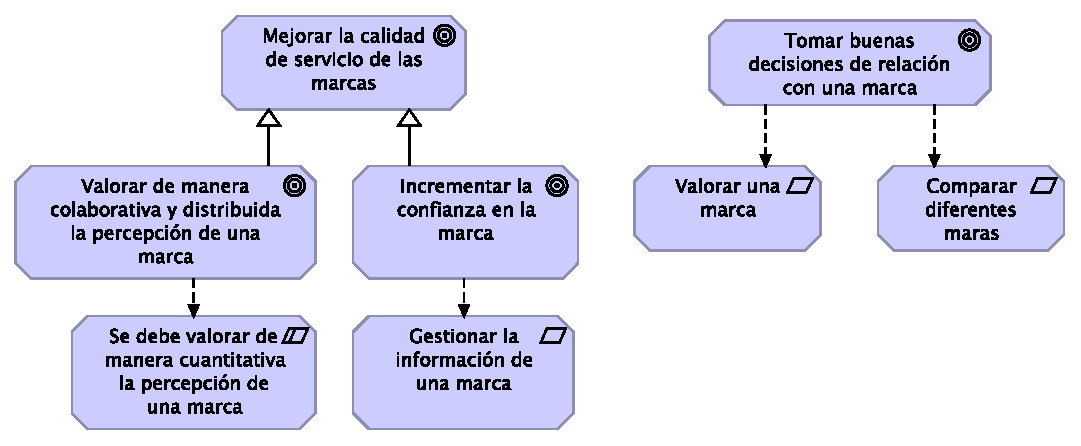
\includegraphics[scale=0.70]{MRealizacionrequerimientos}
\caption{Punto de vista de realización de requisitos.}
\end{figure}


\section{Motivación}
La motivación punto de vista permite al diseñador o analista modelar el aspecto de la motivación, sin centrarse en determinados elementos dentro de este aspecto. Por ejemplo, este punto de vista se puede utilizar para presentar una visión completa o parcial del aspecto motivación en la relación de las partes interesadas, sus objetivos principales, los principios que aplican, y los principales requerimientos de servicios, procesos, aplicaciones y objetos.

\begin{figure}[H]
\centering
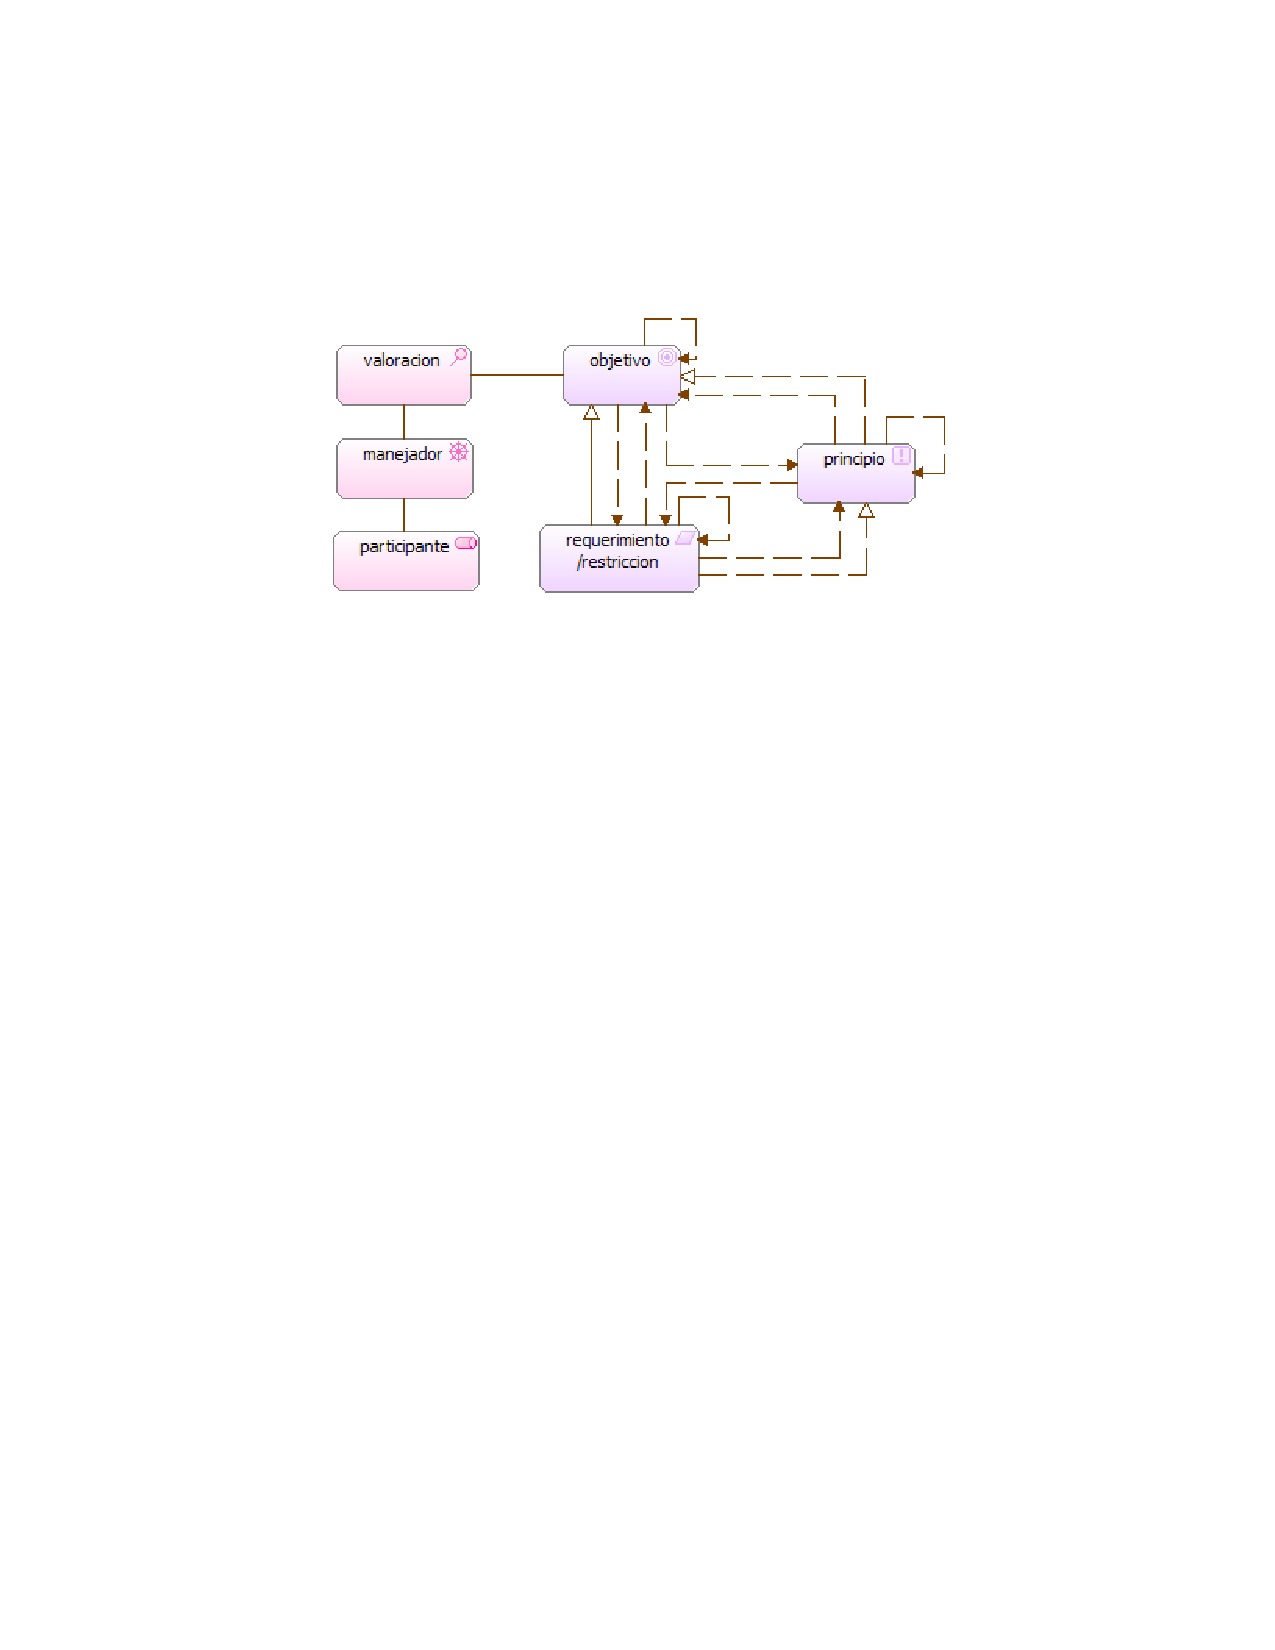
\includegraphics{motivacion}
\caption{Metamodelo del punto de vista de motivación.}
\end{figure}

Se puede observar en la figura del punto de vista de motivación \ref{mmotivacion}, que los manejadores más importantes que deben ser tenidos en cuenta en este negocio son: mejora continua de la marca y satisfacción del usuario. 

\begin{figure}[H]
\centering
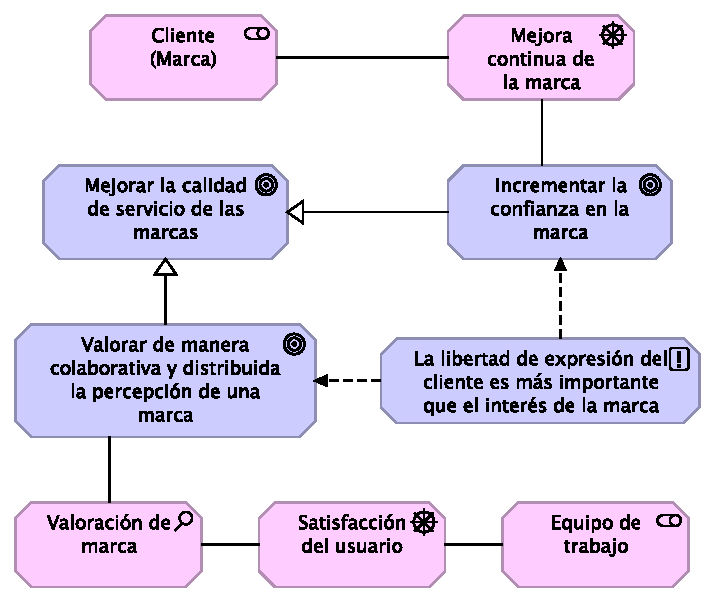
\includegraphics[scale=0.8]{MMotivacion}
\caption{Punto de vista de motivación.}
\label{mmotivacion}
\end{figure}


\section{Proyecto}
Un punto de vista del proyecto se utiliza principalmente para modelar la gestión del cambio de arquitectura. La \textit{arquitectura} del proceso de migración de una vieja situación (estado actual de arquitectura empresarial) a una nueva situación deseada (objetivo de arquitectura de la empresa) tiene consecuencias importantes sobre el subsiguiente proceso de toma de decisiones de la estrategia de crecimiento a largo plazo y medio. 

\begin{figure}[H]
\centering
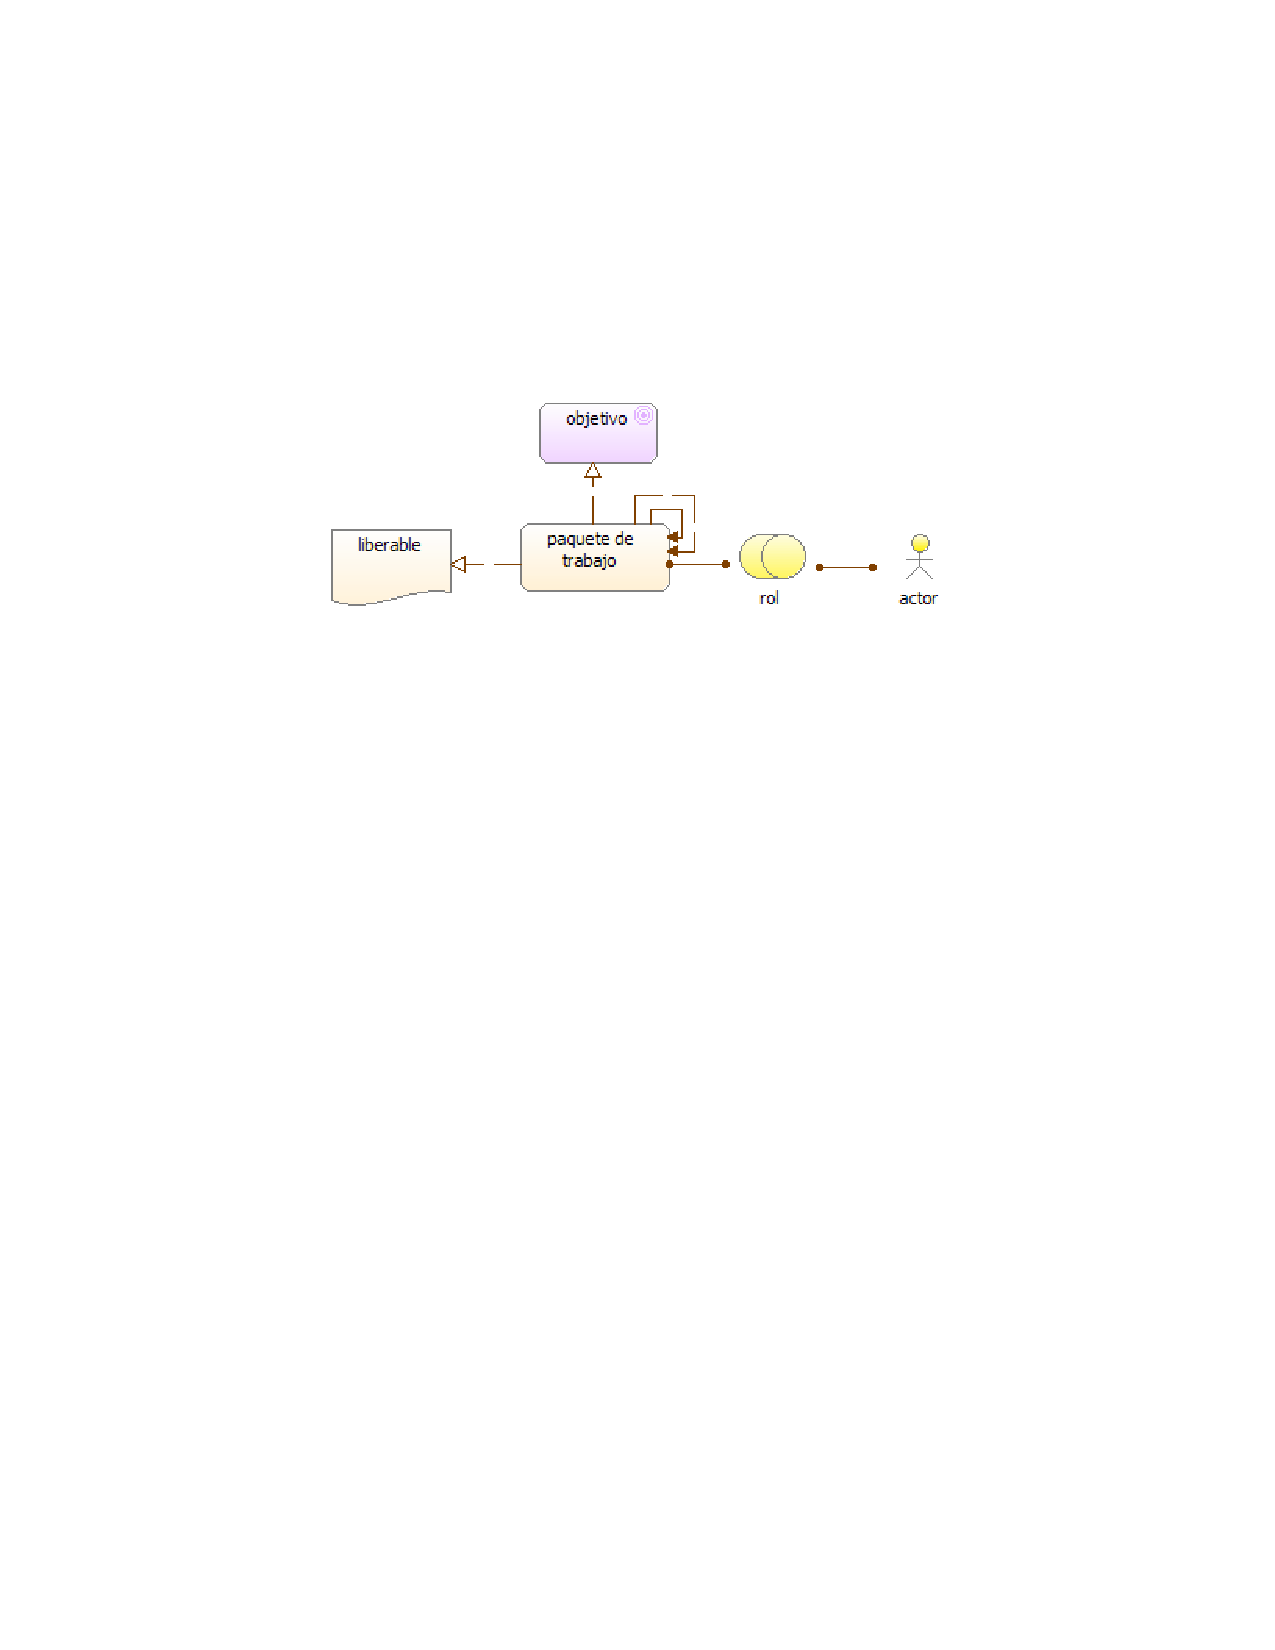
\includegraphics{proyecto}
\caption{Metamodelo del punto de vista de proyecto.}
\end{figure}

Algunas de las decisiones que deben ser tomadas en cuenta por los modelos diseñados en este punto de vista son: 
\begin{itemize}
      \item El desarrollo de la arquitectura empresarial en toda la organización es una tarea que puede requerir varios años. 
        \item Todos los sistemas y servicios deben permanecer en funcionamiento sin tener en cuenta todas las modificaciones y presumibles cambios en la arquitectura de la empresa durante el proceso de cambio. 
        \item El proceso de cambio puede tener que lidiar con los estándares de tecnología inmadura (por ejemplo, mensajería, seguridad, datos, etc.). 
        \item El cambio tiene graves consecuencias para el personal, la cultura, la forma de trabajar y la organización.    
\end{itemize}

Además, hay varios otros aspectos de gobierno, que obstaculizaron el proceso de transformación, tales como la cooperación interna y externa, la gestión de la cartera de proyectos, gestión de proyectos (entregables, objetivos, etc.), la planificación de la platea, los aspectos financieros y legales, etc.

\marginpar{
    \begin{figure}[H]
        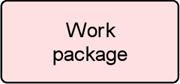
\includegraphics[scale=0.8]{Iwork_package}
    \end{figure} 
    \footnotesize 
    \textbf{Paquete de trabajo}. Una serie de acciones destinadas a lograr un objetivo único dentro de un tiempo especifico.
\newline
}
\marginpar{
    \begin{figure}[H]
        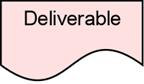
\includegraphics[scale=0.8]{Ideliverable}
    \end{figure} 
    \footnotesize 
    \textbf{Liberable}. Un resultado definido precisamente  de un paquete de trabajo.
}

Este proyecto debe ser inicialmente orientado a la construcción de la aplicación móvil de valoración de marcas con el objetivo de lograr, a partir de la valoración de los usuarios, recoger la información que permita valorar de manera colaborativa y distribuida la percepción de una marca. 

\begin{figure}[H]
\centering
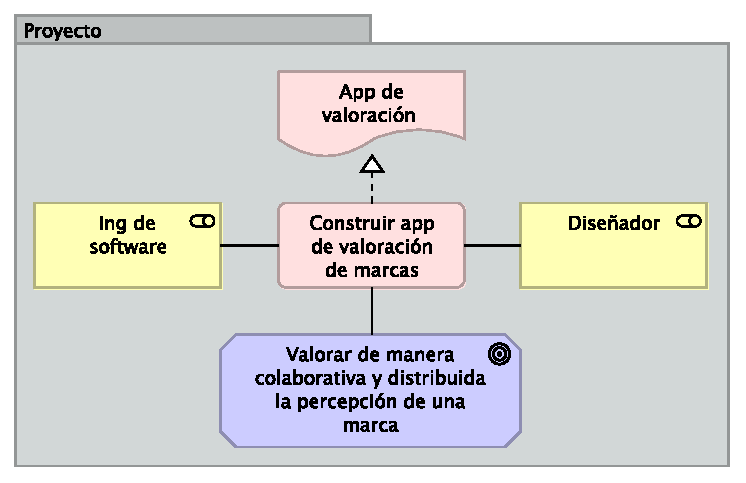
\includegraphics{MProyecto}
\caption{Punto de vista de proyecto.}
\end{figure}

\section{Migración}

El punto de vista de migración implica modelos y conceptos que se pueden utilizar para especificar la transición de una arquitectura existente a una arquitectura deseada.

\begin{figure}[H]
\centering
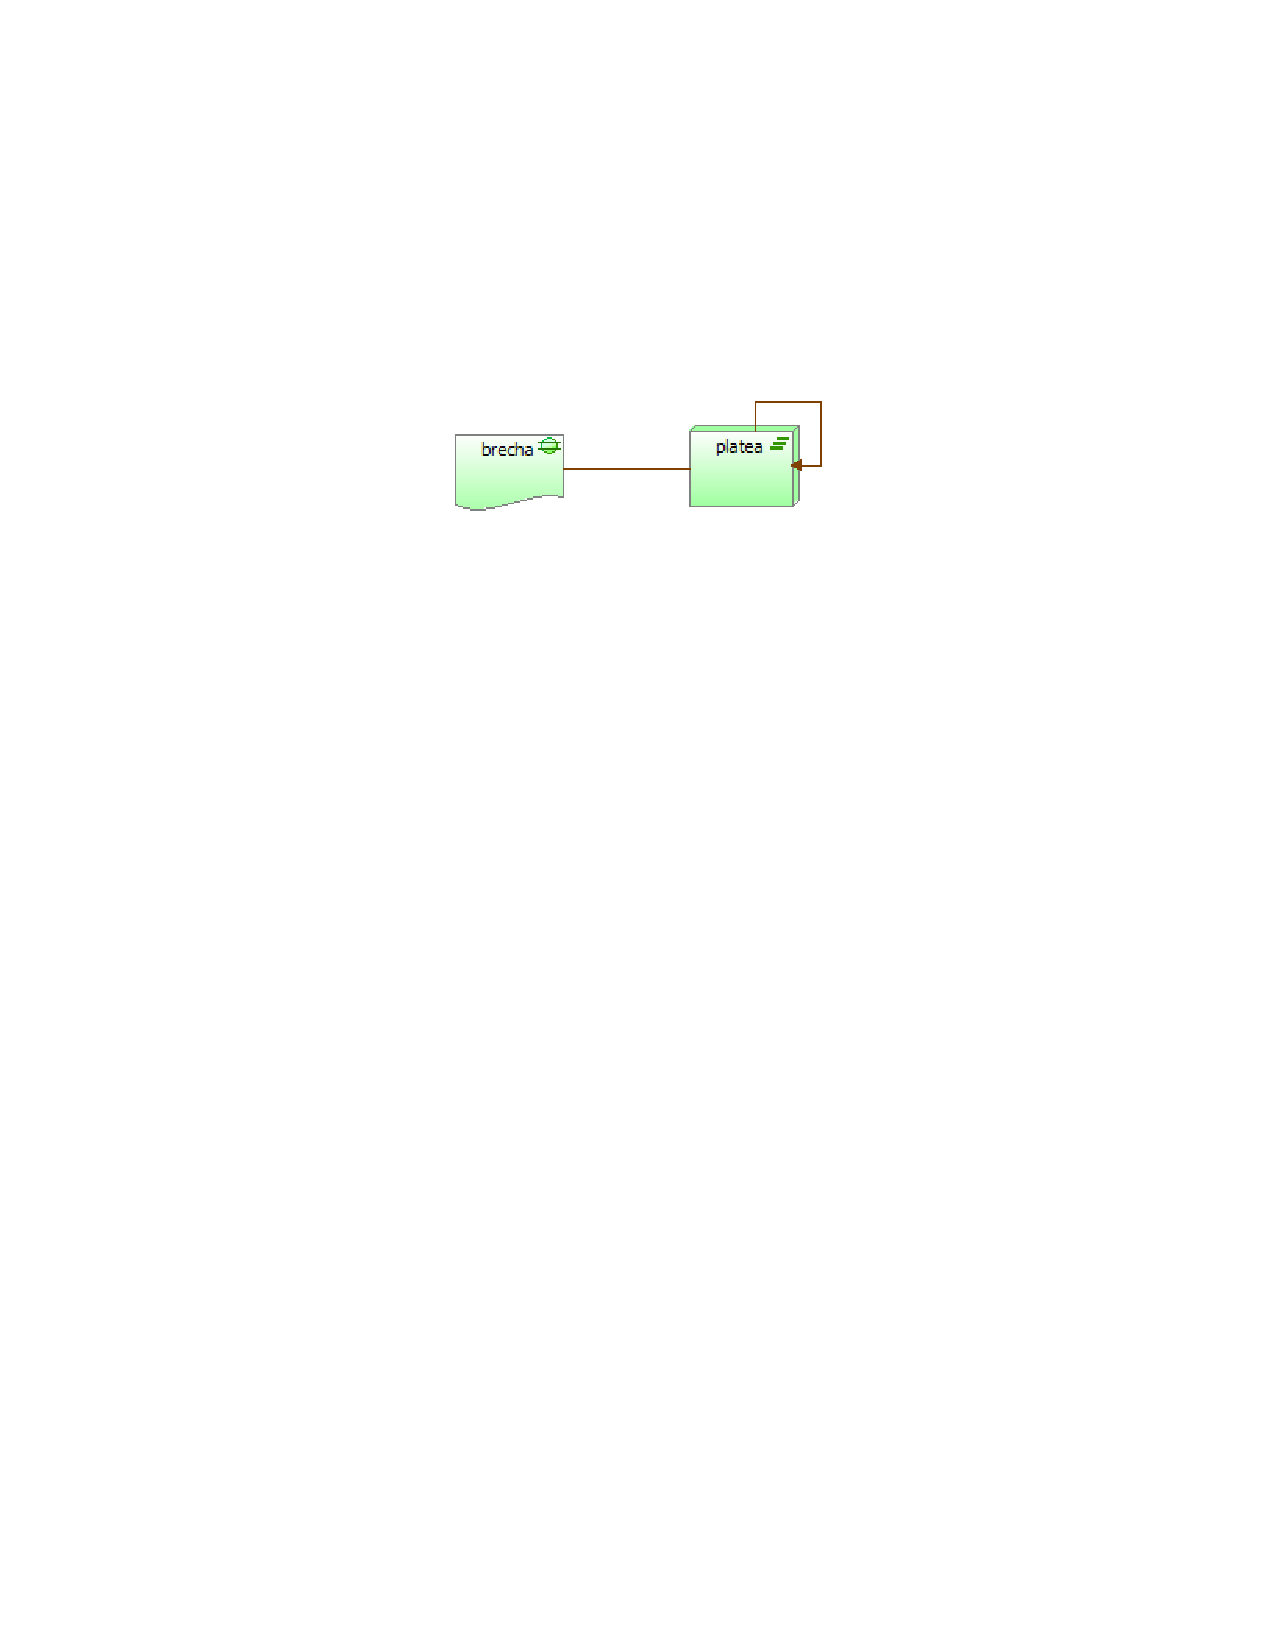
\includegraphics{migracion}
\caption{Metamodelo del punto de vista de migración.}
\end{figure}

\marginpar{
    \begin{figure}[H]
        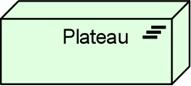
\includegraphics[scale=0.8]{Iplateau}
    \end{figure} 
    \footnotesize 
    \textbf{Platea}. Un estado relativamente estable de la arquitectura que existe durante un período de tiempo limitado.
\newline
}
\marginpar{
    \begin{figure}[H]
        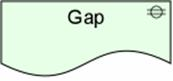
\includegraphics[scale=0.8]{Igap}
    \end{figure} 
    \footnotesize 
    \textbf{Brecha}. Uno de los resultados del análisis de la brecha entre dos plateas. 
}El producto planeado será el sistema software de valoración de marcas, pero adicionalmente se espera escalar en dos grandes plateas. Primero la personalización de ciertas valoraciones y segundo, la comunicación directa entre marcas y usuarios.

\begin{figure}[H]
\centering
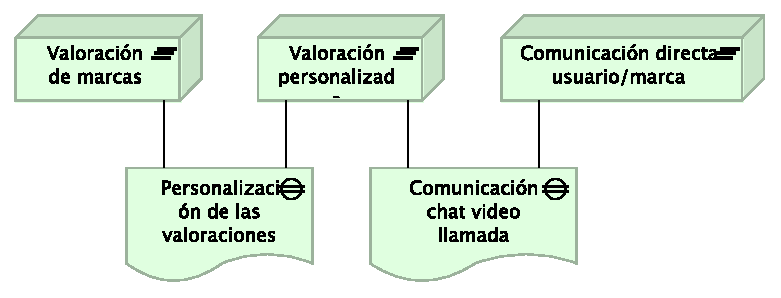
\includegraphics{MMigracion}
\caption{Punto de vista de migración.}
\end{figure}


\section{Migración e implementación}

El punto de vista de la migración y la implementación se utiliza para relacionar los programas y proyectos de las partes de la arquitectura que se implementan. Esta vista permite el modelado del alcance de los programas, proyectos, actividades del proyecto en términos de las plateas que se realizan o los elementos de la arquitectura individuales que se ven afectados. Además, la forma en que se ven afectados los elementos puede ser indicado por la anotación de las relaciones. 

\begin{figure}[H]
\centering
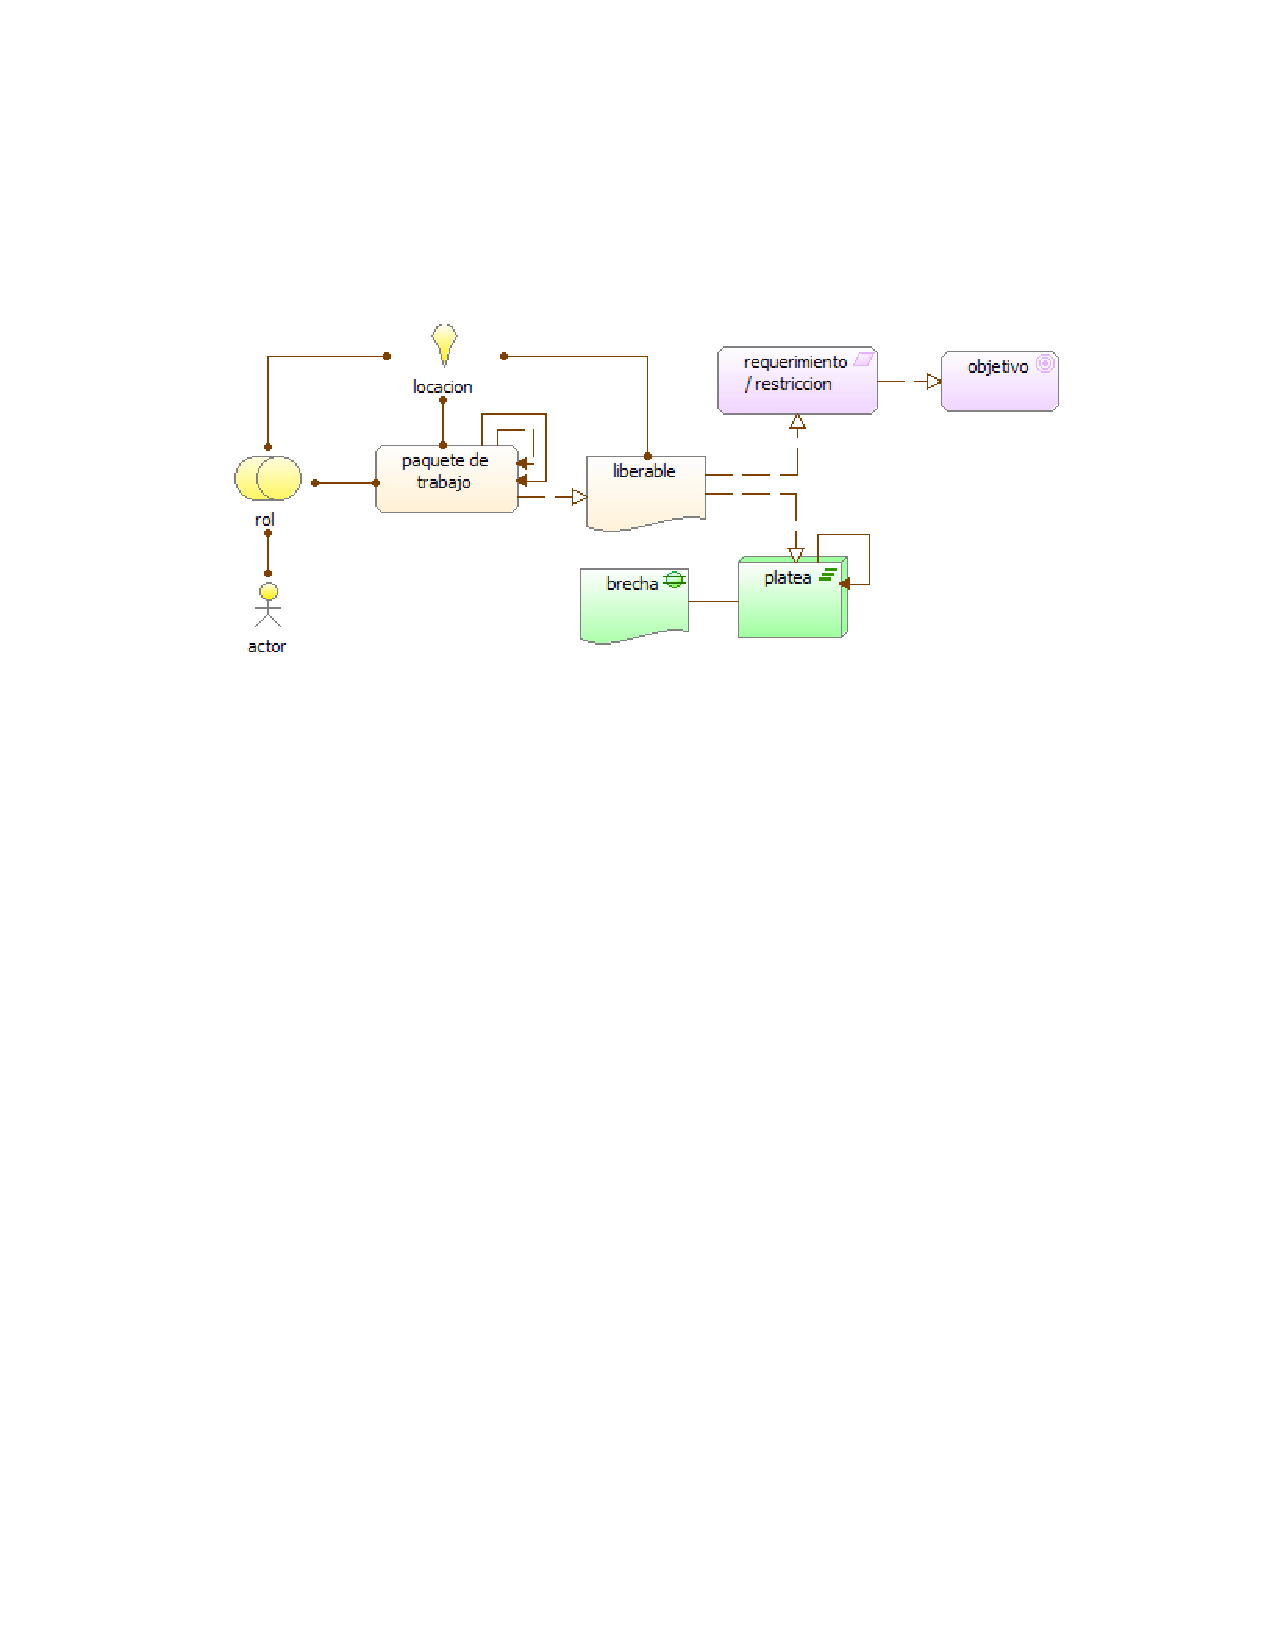
\includegraphics[scale=0.7]{migracion_e_implementacion}
\caption{Metamodelo del punto de vista de migración e implementación.}
\end{figure}

Por otra parte, este punto de vista se puede utilizar en combinación con el punto de vista de los programas y proyectos para apoyar la gestión del portafolio: 
\begin{itemize}
        \item El punto de vista de los programas y proyectos es adecuado para relacionar los objetivos de negocio a los programas y proyectos. Por ejemplo, esto hace posible el análisis a un nivel alto si todos los objetivos de negocio se cubren de manera suficiente por la portafolio actual. 
        \item El punto de vista de la implementación y la migración es adecuado para relacionar los objetivos de negocio (y requisitos) a través de programas y proyectos de (partes de) la arquitectura. Por ejemplo, esto hace posible el análisis de la posible superposición entre las actividades del proyecto o para analizar la coherencia entre las dependencias y las dependencias del proyecto entre las plateas o elementos de la arquitectura.
\end{itemize}

Como realización del objetivo principal con su restricción se debe crear un entregable principal que se materializará como la primera platea.

\begin{figure}[H]
\centering
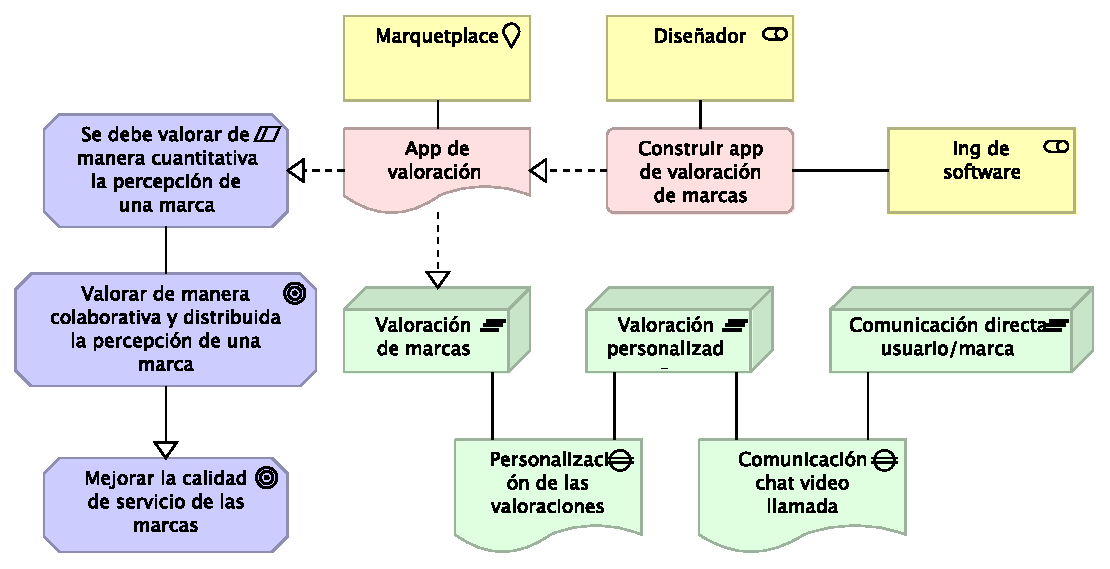
\includegraphics[scale=0.7]{MMigracioneimplementacion}
\caption{Punto de vista de migración e implementación.}
\end{figure}

